\section{Common Distributions}

\subsection{Multivariate Gaussians}

Recall $X \sim \mathcal{N}(\mu, \sigma^2)$ implies that its PDF is 
\[f_X (x) = \frac{1}{\sigma \sqrt{2 \pi}} e^{-\frac{(x - \mu)^2}{2 \sigma^2}}\]
Now we will consider a Gaussian random \textit{vector}, which can be considered a vector of random variables  
\[\mathbf{X} = \begin{bmatrix} X_1 \\ X_2 \\ \vdots \\ X_n \end{bmatrix}\]
mapping from $\Omega$ to $\mathbb{R}^n$. It is not merely a vector where every $X_i$ is Gaussian, as we will show later. That is, a joint distribution that has all $n$ marginal distributions Gaussians does not make a multivariate Gaussian. 

This measurable function $\mathbf{X}: \Omega \rightarrow \mathbb{R}^n$ induces a probability law $\mathbb{P}_X$ on $\mathcal{B}(\mathbb{R}^n)$, and the Radon-Nikodym theorem states the existence of a PDF $f_X$ such that $\mathbb{P}_X (B) = \int_B f_X \,d\lambda$.

\subsubsection{Bivariate Gaussians}
Let us first begin with two-variable Gaussians. 

\begin{definition}[Standard Bivariate Gaussian RV]
A random variable $(X, Y)$ is said to be a \textbf{standard bivariate Gaussian} if its PDF is of form
\[f_{X, Y} (x, y) = \frac{1}{2 \pi \sqrt{1 - \rho^2}} \exp \bigg( -\frac{x^2 - 2 \rho x y + y^2}{2 (1 - \rho^2)} \bigg) \text{ for } \rho \in (-1, 1)\] 
\end{definition}

\begin{theorem}
Given a standard bivariate Gaussian $(X, Y)$, 
\begin{enumerate}
    \item $X$ and $Y$ are marginally distributed as $\mathcal{N}(0, 1)$. That is, if we integrate a variable (say, $x$) out, we will get a univariate standard Gaussian PDF of the other ($y$): 
    \[\int_{-\infty}^\infty \frac{1}{2 \pi \sqrt{1 - \rho^2}} \exp \bigg( -\frac{x^2 - 2 \rho x y + y^2}{2 (1 - \rho^2)}\bigg) \,dx = \frac{1}{\sqrt{2 \pi}} e^{-y^2 / 2}\]
    \item $\rho_{X, Y}$, the correlation coefficient of $X$ and $Y$, is equal to $\rho$. 
    \item The conditional distribution of $X$ given $Y = y$ is $X \mid Y = y \sim \mathcal{N} (\rho y, 1 - \rho^2)$. That is, 
    \[f_{X \mid Y} (x \mid y) = \frac{1}{2 \pi \sqrt{1 - \rho^2}} \exp \bigg( -\frac{x^2 - 2 \rho x y + y^2}{2 (1 - \rho^2)}\bigg) = \frac{1}{ \sqrt{2 \pi (1 - \rho^2)}} \, \exp\bigg( - \frac{(x - (\rho y))^2}{2 (1 - \rho^2)} \bigg)\]
    \item From (3), we can see that the conditional expectation $\mathbb{E}[X \mid Y = y] = \rho y$ since $X \mid Y = y$ has mean at $\rho y$. Therefore, the conditional expectation of $X$ given $Y$ (which is a random variable) is 
    \[\mathbb{E}[X \mid Y] = \rho Y\]
    i.e. $\mathbb{E}[X \mid Y]$ is a linear function of $Y$. 
\end{enumerate}
\end{theorem}

The formula of the general bivariate Gaussian $\mathbf{X} = (X_1, X_2)$ PDF is messy, but we will put it here. 
\[f_{X_1, X_2} (x, y) = \frac{\sigma_1 \sigma_2 \sqrt{1 - \rho^2}} \exp \bigg[ -\frac{1}{2} \bigg( \frac{(x_1 - \mu_1)^2}{\sigma_1^2} + \frac{(x_2 - \mu_2)^2}{\sigma_2^2} - 2 \rho \frac{(x_1 - \mu_1)}{\sigma_1} \frac{(x_2 - \mu_2)}{\sigma_2}\bigg)\bigg]\]
It is cleaner to put it into matrix form. 
\[f_{X_1, X_2} (x_1 , x_2) = \frac{1}{2 \pi \sqrt{\mathrm{det}(\boldsymbol{\Sigma})}} \exp \bigg( - \frac{(\mathbf{x} - \boldsymbol{\mu})^T \boldsymbol{\Sigma}^{-1} (\mathbf{x} - \boldsymbol{\mu})}{2} \bigg) \]
where 
\[\mathbf{x} = \begin{pmatrix} x_1 \\ x_2 \end{pmatrix}, \;\; \boldsymbol{\mu} = \begin{pmatrix} \mu_1 \\ mu_2 \end{pmatrix} , \;\; \boldsymbol{\Sigma} = \mathbb{E}\big[ (\mathbf{X} - \boldsymbol{\mu}) (\mathbf{X} - \boldsymbol{\mu})^T \big] = \begin{pmatrix} \mathrm{Var}(X_1) & \mathrm{Cov}(X_1, X_2) \\
\mathrm{Cov}(X_1, X_2) & \mathrm{Var}(X_2) \end{pmatrix}\]

Note that visually, $\boldsymbol{\Sigma}$ will determine how much the Gaussian distribution is "stretched" on one way or another. Obviously, the "peak" of the distribution will be $\boldsymbol{\mu}$. If $\boldsymbol{\Sigma} = I$, then we could visualize the Gaussian distribution as being perfectly symmetric. However, if we scale the distribution up to a certain constant (below shown $\boldsymbol{\Sigma} = I$, $\boldsymbol{\Sigma} = 0.61 I$, $\boldsymbol{\Sigma} = 2 I$), we get
\begin{center}
    \includegraphics[scale=0.65]{img/Gaussian_Distribution.png}
\end{center}

Now we've made a remark before that given a multivariate distribution $\mathbf{X} = (X_1, \ldots, X_n)$, all of its marginal distributions being Gaussian does not mean that $\mathbf{X}$ is a multivariate Gaussian. We give a counterexample. 

\begin{example}
Let $Y_1, Y_2$ be iid random variables distributed according to the PDF 
\[f_Y (y) = \sqrt{\frac{2}{\pi}} e^{-y^2 / 2} \text{ for } y > 0\]
which we can interpret as a one-sided Gaussian. Let $W \sim \mathrm{Bernoulli}(\frac{1}{2})$ be independent of $Y_1$ and $Y_2$. Now, define the random variables 
\[X_1 = W \, Y_1 \text{ and } X_2 = W \, Y_2\]
This is clearly not a multivariate Gaussian, even though the marginals are $X_1, X_2 \sim \mathcal{N}(0, 1)$. We could make the degenerate case that $X_1 = X_2$, which would make the image of $(X_1, X_2)$ just the line at $x_1 = x_2$, but we can think of this as a degenerate Gaussian with a singular $\boldsymbol{\Sigma}$. 

\begin{figure}[H]
  \centering 
  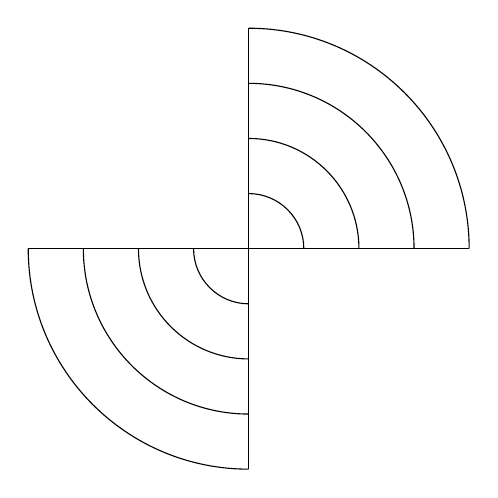
\begin{tikzpicture}[scale=0.7]
    % Draw the x and y axes
    \draw (-4,0) -- (4,0);
    \draw (0,-4) -- (0,4);
    
    \draw (1,0) arc (0:90:1);
    \draw (-1,0) arc (180:270:1);
    \draw (2,0) arc (0:90:2);
    \draw (-2,0) arc (180:270:2);
    \draw (3,0) arc (0:90:3);
    \draw (-3,0) arc (180:270:3);
    \draw (4,0) arc (0:90:4);
    \draw (-4,0) arc (180:270:4);
  \end{tikzpicture}
  \caption{Now note that $Y_1$ and $Y_2$ are both positive, and since $X_1$ and $X_2$ are both dependent on the same value of $W$, it is either $X_1$ and $X_2$ are both positive or both negative. So, the joint distribution of $X_1, X_2$ will be on only the 1st and 3rd quadrant with no mass on the 2nd and 4th. }
  \label{fig:not_multi_gaussian}
\end{figure}
\end{example}

\subsubsection{Multivariate Gaussians}

There are three equivalent definitions of multivariate Gaussians of $n$-variables. 

\begin{definition}[Multivariate Gaussian]
Let us have a vector-valued random variable $\mathbf{X} = (X_1 \ldots X_n)^T \sim \mathcal{N}(\boldsymbol{\mu}, \boldsymbol{\Sigma})$. 
\begin{enumerate}
    \item $\mathbf{X}$ is a \textbf{multivariate Gaussian distribution} with mean $\boldsymbol{\mu} \in \mathbb{R}^n$ and symmetric, positive-definite covariance matrix $\boldsymbol{\Sigma} \in \mathbb{R}^{n \times n}$ if its probability density function is
    \[f_X (x) = \frac{1}{(2\pi)^{n/2} \mathrm{det}(\boldsymbol{\Sigma})^{1/2}} \exp\bigg( -\frac{1}{2} (x-\boldsymbol{\mu})^T \boldsymbol{\Sigma}^{-1} (x - \boldsymbol{\mu})\bigg)\]
    The covariance matrix $\boldsymbol{\Sigma}$ is the $n \times n$ matrix whose $(i, j)$th entry is $\Cov(X_i, X_j)$. That is, for any random vector $\mathbf{X}$ with mean $\boldsymbol{\mu}$, its covariance matrix 
    \[\boldsymbol{\Sigma} = \mathbb{E}\big[ (\mathbf{X} - \boldsymbol{\mu}) (\mathbf{X} - \boldsymbol{\mu})^T \big] = \mathbb{E}[\mathbf{X} \mathbf{X}^T] - \boldsymbol{\mu} \boldsymbol{\mu}^T\]
    is positive definite and symmetric, which implies by the spectral theorem we can break it down into $n$ orthogonal eigenspaces of positive eigenvalues. 

    \item $X$ is a multivariate Gaussian distribution if it can be expressed as 
    \[\mathbf{X} = \mathbf{D} \mathbf{w} + \boldsymbol{\mu}\]
    where $\mathbf{w}$ is a vector of independent $\mathcal{N}(0, 1)$ Gaussians, $\boldsymbol{\mu} \in \mathbb{R}^n$, and $\mathbf{D} \in \mathbb{R}^{n \times n}$. The mean of $\mathbf{X}$ is $\boldsymbol{\mu}$ and its covariance is $\boldsymbol{\Sigma} = \mathbf{D} \mathbf{D}^T$; $\mathbf{D}$ is called the \textbf{standard deviation matrix}. When modeling high-dimensional Gaussians, this way is most computationally feasible. 

    \item $X$ is a multivariate Gaussian distribution if for every $\mathbf{a} \in \mathbb{R}^n$, $\mathbf{a}^T \mathbf{x}$ is a Gaussian RV. This means that if we take $\mathbf{a} = \mathbf{0}$, then the entire $\mathbf{X}$ is constantly $0$, which we will take to be the degenerate Gaussian with mean, variance $0$. 
\end{enumerate}
The $n$ semi-axes of the $(n-1)$-dimensional isocontour ellipsoid formed by an $n$-dimensional Gaussian distribution are precisely the normalized eigenvectors of $\boldsymbol{\Sigma}$ multiplied by their eigenvalues. 
\end{definition}


If we let $\boldsymbol{\Sigma} = \mathbf{I}$, then this means that all the $X_i$'s are pairwise uncorrelated since $\Sigma_{ij} = \Cov (X_i, X_j) = 0$. In general, this does not mean that the $X_i$'s are independent, but for joint Gaussians, this also implies independence! 

\begin{theorem}
Given multivariate Gaussian $\mathbf{X} = (X_1 \ldots X_n)^T \sim \mathcal{N}(\boldsymbol{\mu}, \boldsymbol{\Sigma})$, the $X_i$'s are pairwise independent if and only if they are uncorrelated. 
\end{theorem}
\begin{proof}
We can expand the PDF of $\mathbf{X}$ as 
\begin{align*}
    f_X (x) & = \frac{1}{(2 \pi)^{n/2}} \exp \bigg( -\frac{1}{2} (x - \mu)^T (x - \mu) \bigg) \\
    & = \bigg(\frac{1}{\sqrt{2\pi}} \bigg)^n \exp \bigg( \sum_{i=1}^n -\frac{1}{2} (x_i - \mu_i)^2 \bigg) \\
    & = \prod_{i=1}^n \frac{1}{\sqrt{2\pi}} \exp \bigg( -\frac{1}{2} (x_i - \mu_i)^2 \bigg)
\end{align*}
which is the product of $n$ single-variable Gaussians $X_i$. Therefore this means that independence and uncorrelation are equivalent! 
\end{proof}

Therefore, if the nondiagonal entries of the covariance matrix are all $0$, then we know that the variables are all uncorrelated and therefore independent. 

